\documentclass[10pt]{beamer}
\usepackage[utf8x]{inputenc}
\usepackage{hyperref}
\usepackage{fontawesome}
\usepackage{graphicx}
\usepackage[croatian]{babel}

% ------------------------------------------------------------------------------
% Use the beautiful metropolis beamer template
% ------------------------------------------------------------------------------
\usepackage[T1]{fontenc}
\usepackage{fontawesome}
\usepackage{FiraSans} 
\mode<presentation>
{
  \usetheme[progressbar=foot,numbering=fraction,background=light]{metropolis} 
  \usecolortheme{default} % or try albatross, beaver, crane, ...
  \usefonttheme{default}  % or try serif, structurebold, ...
  \setbeamertemplate{navigation symbols}{}
  \setbeamertemplate{caption}[numbered]
  %\setbeamertemplate{frame footer}{My custom footer}
} 

% ------------------------------------------------------------------------------
% beamer doesn't have texttt defined, but I usually want it anyway
% ------------------------------------------------------------------------------
\let\textttorig\texttt
\renewcommand<>{\texttt}[1]{%
  \only#2{\textttorig{#1}}%
}

% ------------------------------------------------------------------------------
% minted
% ------------------------------------------------------------------------------
\usepackage{minted}


% ------------------------------------------------------------------------------
% tcolorbox / tcblisting
% ------------------------------------------------------------------------------
\usepackage{xcolor}
\definecolor{codecolor}{HTML}{FFC300}

\usepackage{tcolorbox}
\tcbuselibrary{most,listingsutf8,minted}

\tcbset{tcbox width=auto,left=1mm,top=1mm,bottom=1mm,
right=1mm,boxsep=1mm,middle=1pt}

\newtcblisting{myr}[1]{colback=codecolor!5,colframe=codecolor!80!black,listing only, 
minted options={numbers=left, style=tcblatex,fontsize=\tiny,breaklines,autogobble,linenos,numbersep=3mm},
left=5mm,enhanced,
title=#1, fonttitle=\bfseries,
listing engine=minted,minted language=r}


% ------------------------------------------------------------------------------
% Listings
% ------------------------------------------------------------------------------
\definecolor{mygreen}{HTML}{37980D}
\definecolor{myblue}{HTML}{0D089F}
\definecolor{myred}{HTML}{98290D}

\usepackage{listings}

% the following is optional to configure custom highlighting
\lstdefinelanguage{XML}
{
  morestring=[b]",
  morecomment=[s]{<!--}{-->},
  morestring=[s]{>}{<},
  morekeywords={ref,xmlns,version,type,canonicalRef,metr,real,target}% list your attributes here
}

\lstdefinestyle{myxml}{
language=XML,
showspaces=false,
showtabs=false,
basicstyle=\ttfamily,
columns=fullflexible,
breaklines=true,
showstringspaces=false,
breakatwhitespace=true,
escapeinside={(*@}{@*)},
basicstyle=\color{mygreen}\ttfamily,%\footnotesize,
stringstyle=\color{myred},
commentstyle=\color{myblue}\upshape,
keywordstyle=\color{myblue}\bfseries,
}


% ------------------------------------------------------------------------------
% The Document
% ------------------------------------------------------------------------------
\title{Spiza.hr}
\subtitle{Prirodoslovno--matematički fakultet}
\author{Martina Gaćina, Manuela Pleša, Fran Vojković, Alen Živković}
\date{U Zagrebu, \today}

\begin{document}

\maketitle

\section{Uvod}

\begin{frame}[fragile,allowframebreaks]{Uvod}
\begin{itemize}
    \item Napravili smo web-aplikaciju za naručivanje i dostavljanje hrane
\end{itemize}
\begin{figure}[htbp]
            \centerline{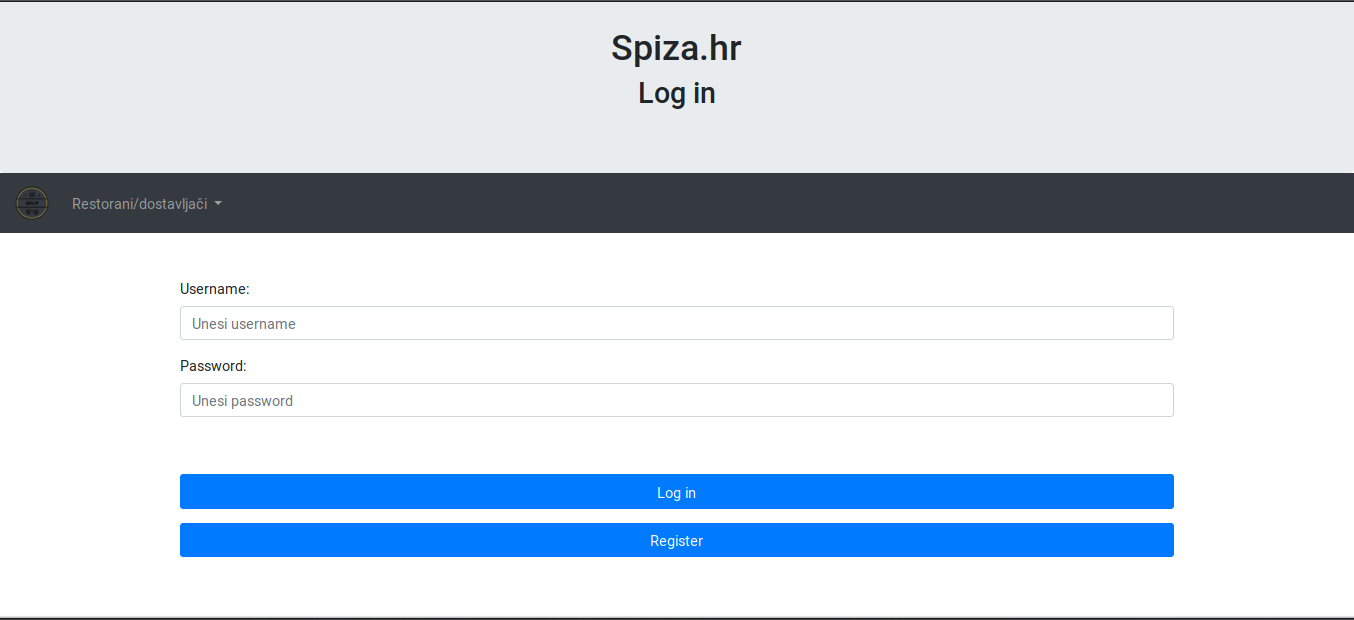
\includegraphics[scale=0.17]{log_in.png}}
            \caption{Log in aplikacije Spiza.hr}
            \label{fig:log_in}
\end{figure}
\framebreak
\begin{itemize}
    \item Vodili smo se poznatim aplikacijama poput Glovo, Wolt ili Pauza.hr
    \item Morali smo čuvati podatke o korisnicima, restoranima, narudžbama, hrani koju restorani imaju u ponudi i povratnoj informaciji korisnika o kvaliteti pa koristimo MySQL bazu podataka
    \end{itemize}

\end{frame}

\section{Baza podataka}

\begin{frame}[fragile,allowframebreaks]{Baza podataka}
Tablice koje koistimo u bazi podataka:
\begin{itemize}
    \item\textsf{USERS} - podaci o korisnicima koji su već registrirani i koji se naknadno registriraju 
    \item\textsf{RESTAURANTS} - svi registrirani restorani 
    \item\textsf{FOOD} - tablica sa svom postupnom hranom u aplikaciji 
    \item\textsf{FOOD\_TYPE} - vrste jela kakve restorani nude 
    \item\textsf{ORDERS} - sve narudžbe, odnosno one tek poslane, dostavljene ili koje se dostavljaju 
\end{itemize}
\framebreak

\begin{itemize}
    \item\textsf{CONTAINS} - što je sve u narudžbi 
    \item\textsf{HAS\_FOODTYPE} - koji restoran nudi kaku vrstu jela  
    \item\textsf{IMAGE} - tablica za korištene slike u aplikaciji
    \item\textsf{DELIVERER} - svi dostavljači 
    \item\textsf{NEIGHBORHOOD} - popis kvartova grada Zagreba gdje se sve nalaze registrirani restorani 
\end{itemize}
\end{frame}


\section{Korisnici}

\begin{frame}[fragile,allowframebreaks]{Korisnici}

\begin{itemize}
    \item Ulogiravanje već postojećeg korisnika ili ako prvi puta koristi aplikaciju, registracija novog korisnika 
    \item Nakon \emph{log in}-a korisnik dobiva popis svojih omiljenih restorana, prema ocjenama kojima ih je ocijenio
\end{itemize}
\framebreak

\begin{figure}[htbp]
            \centerline{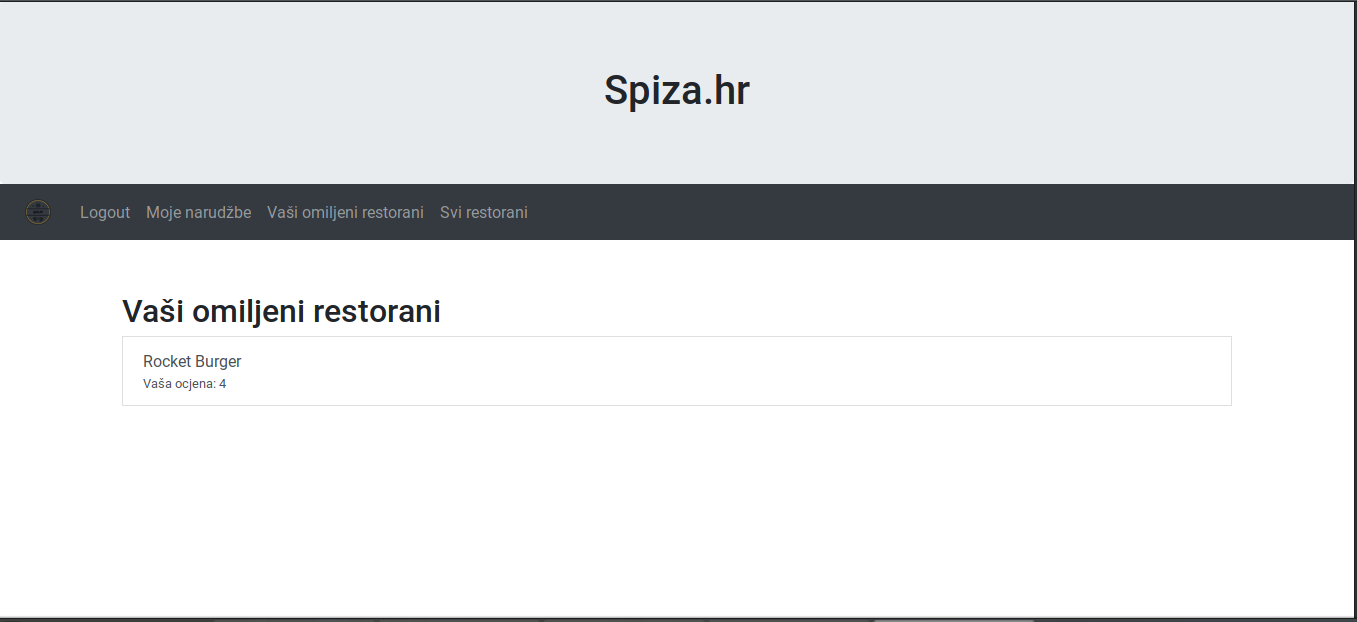
\includegraphics[scale=0.23]{user_naslovna.png}}
            \caption{Naslovna stranica korisnika}
            \label{fig:user}
\end{figure}
\framebreak
\begin{itemize}
    \item\emph{Moje narudžbe} - popis svih korisnikovih već dostavljenih ili trenutno aktivnih narudžbi
    \item\emph{Vaši omiljeni restorani} - popis restorana opadajuće prema ocjenama tog korisnika koji je kliknuo
    \item\emph{Svi restorani} - svi dostupni restorana i mogućnost kategoriziranja restorana
    \begin{itemize}
        \item\emph{Popularni} - popis resorana opadajuće prema ocjenama svih korisnika
        \item\emph{Svi restorani}
        \item\emph{U kvartu} - korisnik odabire kvart koji ga zanima i dobiva popis restorana u tom kvartu
        \item\emph{Prema vrsti hrane} - korisnik bira koju vrstu hrane želi i dobije popis restorana s tom vrstom hrane
     \end{itemize}
\end{itemize}

\end{frame}

\begin{frame}[fragile,allowframebreaks]{Naručivanje}
\begin{enumerate}
    \item Odabir restorana
    \item Odabir jela (1 ili više)
    \item Ulazak u košaricu gdje se naknadno može povećati količina pojedinog jela
    \item Klikom na \emph{Naruči} potrebno je ispuniti podatke o narudžbi te kliknuti \emph{Pošalji narudžbu}
    \item Ulaskom u košaricu u svakom trenu je dostupan gumb \emph{Odbaci narudžbu} kojom odustajete od narudžbe
    \item Korisnik dobije obavijest gdje može pratiti u kojoj fazi je narudžba
\end{enumerate}
\begin{figure}[htbp]
            \centerline{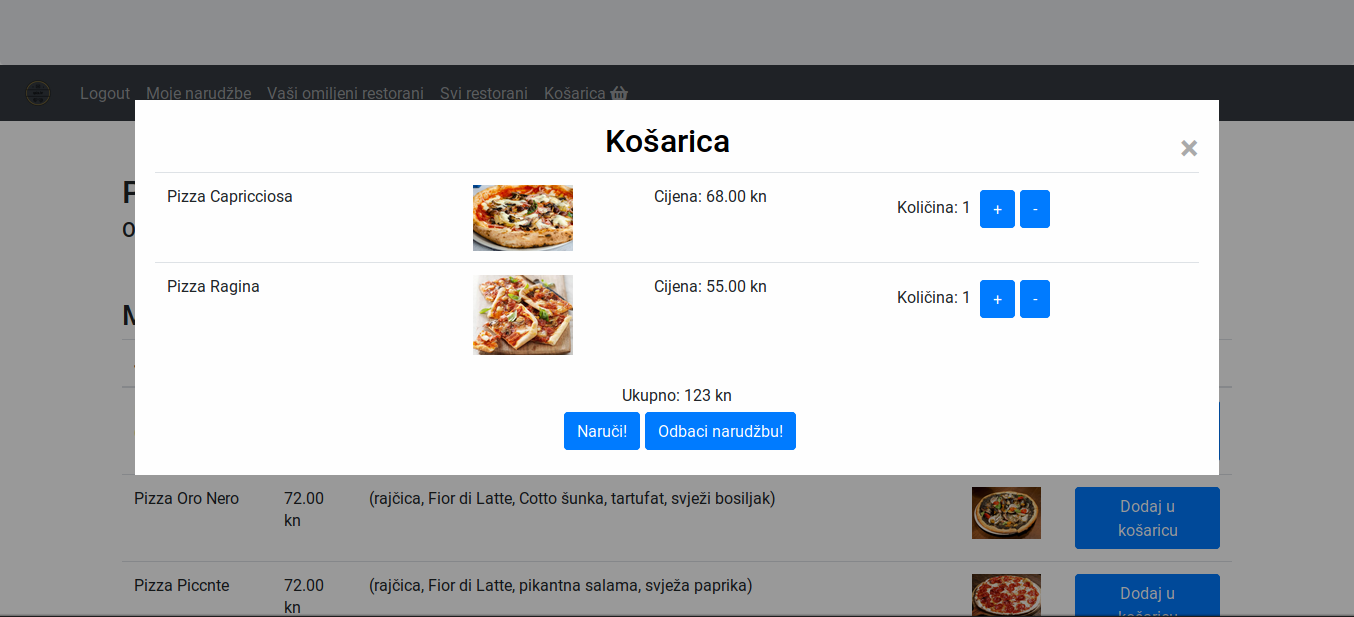
\includegraphics[scale=0.23]{user_kosarica.png}}
            \caption{Košarica}
            \label{fig:user}
\end{figure}
\end{frame}

\section{Restorani}

\begin{frame}[fragile,allowframebreaks]{Restorani}
\begin{itemize}
    \item\emph{log in} već postojećih restorana ili registriranje novih restorana
    \item\emph{Naslovnica}
    \begin{itemize}
        \item Popis trenutnih aktivnih narudžbi tog restorana te gumbi
        \begin{enumerate}
            \item\emph{Prihvati narudžbu} - prije toga je potrebno unijeti vrijeme pripreme te narudžbe
            \item\emph{Odbij narudžbu}
        \end{enumerate}
        \item Menu koji nudi
        \item\emph{Uredi jelo} - mogućnost mijenjanja podataka o nekom jelu
        \item Podaci o restoranu
        \item\emph{Promijeni detalje} - mogućnost mijenjanja podataka o restoranu
        \end{itemize}
    \item\emph{Prošle narudžbe} - popis svih narudžbi koje je taj restoran zaprimio
\end{itemize}

\begin{figure}[htbp]
            \centerline{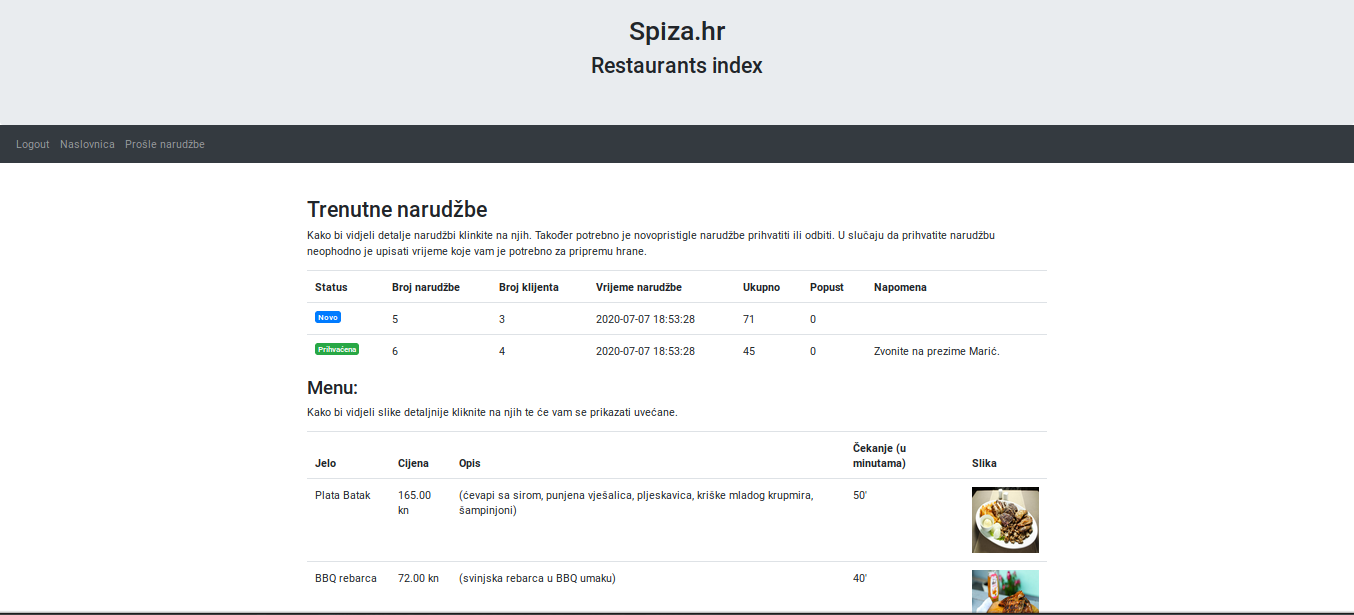
\includegraphics[scale=0.23]{restaurant_naslovna.png}}
            \caption{Naslovnica restorana}
            \label{fig:restaurant}
\end{figure}

\end{frame}

\section{Dostavljači}

\begin{frame}[fragile,allowframebreaks]{Dostavljači}
\begin{itemize}
    \item\emph{Naslovnica} - popis trenutno slobodnih nedostavljenih narudžbi
    \item Prihvaćanje narudžbe
    \begin{enumerate}
        \item Odabere narudžbu
        \item Unese koliko vremena treba za dostavu
        \item Klikne \emph{Prihvati narudžbu}
    \end{enumerate}
    \item\emph{Aktivne narudžbe}
    \begin{itemize}
        \item Prikaže narudžbu koju dostavljač u tom trenutku dostavlja ako ona postoji
        \item Kada završi s dostavom
        \begin{enumerate}
            \item Označi da je dostava gotova
            \item klik na \emph{Dostavljeno}
        \end{enumerate}
    \end{itemize}
\end{itemize}
\framebreak
\begin{figure}[htbp]
            \centerline{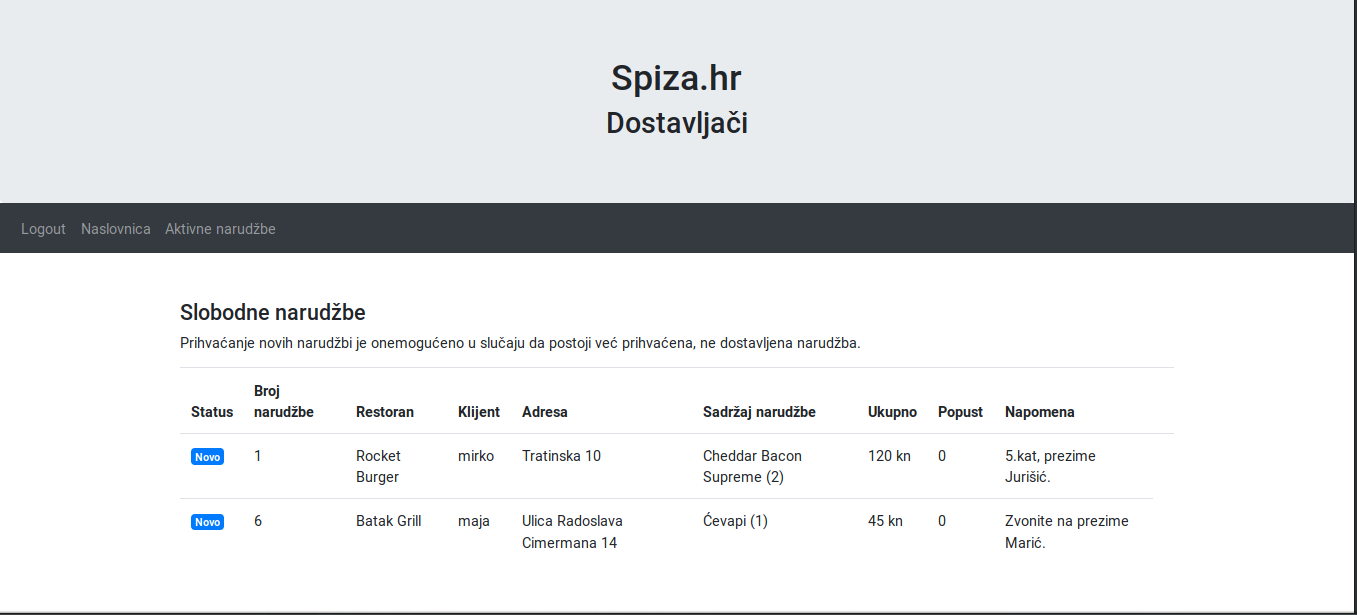
\includegraphics[scale=0.23]{deliverer_naslovna.png}}
            \caption{Naslovnica dostavljača}
            \label{fig:deliverer}
\end{figure}
\end{frame}

\begin{frame}[standout]
    Hvala na pozornosti ~\alert{\faSmileO}~
\end{frame}

\end{document}
